% \documentclass{report}
% 
% \usepackage{fancyhdr}
\usepackage{fourier-orns}
\usepackage{hyperref}%% To refrence links / jumps
\usepackage{chngcntr} %% For some extra counters numberings
\usepackage[a4paper, right = 0.5in, left = 0.5in,top = 1in , bottom = 1in]{geometry}
\usepackage{etoolbox} %% Provides like a language for advanced customization
\usepackage{datetime} %% For dates of course
\usepackage{lastpage} %% provides pages numbers
\usepackage[sc]{titlesec} %% modify titles
\usepackage{enumerate}
\usepackage{cancel}
\usepackage{tikzsymbols}
\usepackage[dvipsnames]{xcolor}
\usepackage{import}
\usepackage{pdfpages} %% include other pdfs
\usepackage{transparent} %% Transparency
\usepackage{xcolor}  %% Colors
\usepackage[many]{tcolorbox}
\usepackage[framemethod=TikZ]{mdframed}
\usepackage{amsmath,amsfonts,amsthm,amssymb,mathtools}
\usepackage{tikz}
\usepackage{bookmark}
\usepackage{graphicx}
\usepackage{mathpazo}

\usepackage{fontawesome5}

\linespread{1.5}


\titleformat{\chapter}[display]   
{\fontfamily{ppl}\selectfont\huge\color{YellowOrange!80!orange}} % Font style and size 
{\raggedleft\color{purple}\fontsize{70}{0pt}\selectfont\thechapter}   
{-1.5cm}    			                          % Space between the chapter number and title
{
	\begin{tikzpicture}[overlay]
		\node[anchor = west,yshift = 0.2cm,xshift = -1cm] {\fontsize{90}{20} $\int_{}^{} $};
		\node[yshift = 4cm, xshift = 17cm]   {\includegraphics[width = 4cm]{preview0}};
	\end{tikzpicture}
\hspace{1cm}\Huge\raggedright\MakeUppercase}

\titleformat{\section}[block]
{
\fontfamily{ppl}\selectfont\huge\color{YellowOrange!80!orange}
}
{
\color{purple}\fontsize{20}{0pt}\selectfont\thesection 
}
{0cm}
{
	\begin{tikzpicture}[overlay]
		\node[anchor = west,yshift = 0.2cm,xshift = -0.4cm, circle = 1pt] {};
	\end{tikzpicture}
}

\titlespacing*{\section}{0pt}{0.7cm}{1.5cm}


\newcommand{\divider}
{
	\begin{center}
	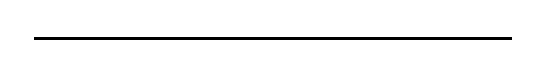
\begin{tikzpicture}
		\draw[thick, black] (0.25*\textwidth, 0) -- (0.75*\textwidth, 0);
		\node[rotate = 360 - 90, xshift = -0.6pt, yshift = 1pt] at (0.25*\textwidth,0){\decotwo};
		\node[rotate = 90, xshift = -0.6pt, yshift = 1pt] at (0.75*\textwidth,0){\decotwo};
	\end{tikzpicture}
	\end{center}
}

\pagestyle{fancy}

\newcommand{\lecday}[1][]
{
    \def\datee{#1}
    \fancyhead[L]{\datee}
}



\newcommand{\signature}
{
	\begin{tikzpicture}[remember picture,overlay]
		\node[fill = YellowOrange!20!white] at ([yshift = 1cm, xshift = -3cm]current page.south east) {\fontsize{10pt}{0pt}{\itshape Kara.$\mathcal{A}$}};
	\end{tikzpicture}
}

\AddToHook{shipout/background}{
  \begin{tikzpicture}[remember picture, overlay]
	  \node[] at ([yshift = 1.5cm,xshift = \textwidth /2 + 0.9cm]current page.south west) {\includegraphics[width = 0.5cm]{preview3}};
	  \node[] at ([yshift = 1.5cm,xshift = - \textwidth /2 - 0.9cm]current page.south east) {\includegraphics[width = 0.5cm]{preview4}};
  \end{tikzpicture}
}



\newtcolorbox[auto counter, number within = section]{remark}[1][]
{
       		title = Remark #1,
		enhanced,
		boxrule = 0pt,
		colback = white,
		breakable,
		arc = 4pt,
		colbacktitle = cyan,
		colback = cyan!5!white,
		segmentation style =
		{
			solid,cyan,thick,
		},
		attach boxed title to top left =
		{
			xshift = 0cm,
		},
		boxed title style =
		{
			boxrule = 0pt,
			sharp corners,
			drop fuzzy shadow = {cyan},
		},
		drop fuzzy shadow = {cyan!80!black},
}

\newtcolorbox[auto counter, number within = section]{theorem}[1][]
{                                      
		title = Theorem \thetcbcounter : #1,
		enhanced, 
		boxrule = 0pt,
		colback = white,
		breakable,
		arc = 4pt,
		colbacktitle = purple,
		colback = purple!5!white,
		segmentation style = 
		{
			solid, purple,thick,
		},
		attach boxed title to top left = 
		{
			xshift = 0cm, 
		},
		boxed title style = 
		{
			boxrule = 0pt,
			sharp corners,
			drop fuzzy shadow = {purple},
		},
		drop fuzzy shadow = {purple!80!black},
}

\newtcolorbox[auto counter, number within = section]{definition}[1][]
{                                      
		title = Definition \thetcbcounter : #1,
		enhanced, 
		boxrule = 0pt,
		colback = white,
		arc = 4pt,
		breakable,
		colbacktitle = YellowOrange!80!black,
		segmentation style = 
		{
			solid, YellowOrange,thick,
		},
		attach boxed title to top left = 
		{
			xshift = 0cm, 
		},
		colback = YellowOrange!5!white,
		boxed title style = 
		{
			boxrule = 0pt,
			sharp corners,
			drop fuzzy shadow = {YellowOrange!80!orange},
		},
		drop fuzzy shadow = {YellowOrange!80!black},
}

\newtcolorbox[auto counter, number within = section]{corollary}[1][]
{                                      
		title = corollary \thetcbcounter : #1,
		enhanced, 
		boxrule = 0pt,
		colback = white,
		arc = 4pt,
		breakable,
		colbacktitle = YellowOrange!80!black,
		segmentation style = 
		{
			solid, YellowOrange,thick,
		},
		attach boxed title to top left = 
		{
			xshift = 0cm, 
		},
		colback = YellowOrange!5!white,
		boxed title style = 
		{
			boxrule = 0pt,
			sharp corners,
			drop fuzzy shadow = {YellowOrange!80!orange},
		},
		drop fuzzy shadow = {YellowOrange!80!black},
}


\newtcolorbox{example}[1][]
{                                      
		title = Example,
		enhanced, 
		boxrule = 0pt,
		colback = white,
		arc = 4pt,
		segmentation style = 
		{
			solid, SpringGreen,thick,
		},
		breakable,
		colback = SpringGreen!5!white,
		colbacktitle = SpringGreen!80!black,
		attach boxed title to top left = 
		{
			xshift = 0cm, 
		},
		boxed title style = 
		{
			boxrule = 0pt,
			sharp corners,
			drop fuzzy shadow = {SpringGreen!80!orange},
		},
		drop fuzzy shadow = {SpringGreen!80!black},
}


\newcommand{\integral}[4]{\int\limits_{#1}^{#2} #4 d#3}
\newcommand{\limit}[3]{\lim\limits_{#1 \rightarrow #2} #3}
\newcommand{\strone}[2]{\left[ \begin{gathered}#1\\ #2\end{gathered} \right] }
\newcommand{\strtwo}[2]{\left\{ \begin{gathered}#1\\ #2\end{gathered} \right\} }
\newcommand{\strthree}[2]{\left\lfloor \begin{gathered}#1\\ #2\end{gathered} \right\rfloor }


\newcommand{\startbf}[1]{\text{\bfseries{#1}}}
\newcommand{\sett}[1]{\left\{ #1 \right\}}
\newcommand{\thesis}[1]{\left( #1 \right)}
\newcommand{\brkt}[1]{\left[ #1 \right]}
\newcommand{\floor}[1]{\left\lfloor #1 \right\rfloor}


\DeclareMathOperator{\img}{im} % Image
\DeclareMathOperator{\Img}{Im} % Image
\DeclareMathOperator{\coker}{coker} % Cokernel
\DeclareMathOperator{\Coker}{Coker} % Cokernel
\DeclareMathOperator{\Ker}{Ker} % Kernel
\DeclareMathOperator{\rank}{rank}
\DeclareMathOperator{\Spec}{Spec} % spectrum
\DeclareMathOperator{\Tr}{Tr} % trace
\DeclareMathOperator{\pr}{pr} % projection
\DeclareMathOperator{\ext}{ext} % extension
\DeclareMathOperator{\pred}{pred} % predecessor
\DeclareMathOperator{\dom}{dom} % domain
\DeclareMathOperator{\ran}{ran} % range
\DeclareMathOperator{\Hom}{Hom} % homomorphism
\DeclareMathOperator{\Mor}{Mor} % morphisms
\DeclareMathOperator{\End}{End} % endomorphism


\newcommand{\lm}{\ensuremath{\lambda}}
\newcommand{\eps}{\ensuremath{\epsilon}}
\newcommand{\veps}{\ensuremath{\varepsilon}}
\newcommand{\al}{\ensuremath{\alpha}}
\newcommand{\bb}{\ensuremath{\beta}}
\newcommand{\cc}{\ensuremath{\gamma}}
\newcommand{\dd}{\ensuremath{\delta}}
\newcommand{\DD}{\ensuremath{\Delta}}
\newcommand{\ff}{\ensuremath{\phi}}
\newcommand{\FF}{\ensuremath{\varphi}}

\newcommand{\RR}{\mathbb{R}}
\newcommand{\RO}{\mathcal{R}}
\newcommand{\EE}{\mathbb{E}}
\newcommand{\CC}{\mathbb{C}}
\newcommand{\RW}{\mathbb{R}^2}
\newcommand{\RT}{\mathbb{R}^3}
\newcommand{\RN}{\mathbb{R}^n}
\newcommand{\DS}{\mathcal{D}}

\newcommand{\KK}{\mathbb{K}}
\newcommand{\KW}{\mathbb{K}^2}
\newcommand{\KT}{\mathbb{K}^3}
\newcommand{\KN}{\mathbb{K}^n}

\newcommand{\NN}{\mathbb{N}}

\newcommand{\PS}{\mathcal{P}}
\newcommand{\AS}{\mathcal{E}}
\newcommand{\FS}{\mathcal{F}}
\newcommand{\LS}{\mathcal{L}}
\newcommand{\MS}{\mathcal{M}}


















\lecday[2025-02-25]

% \begin{document}
\begin{definition}[]
Let $E $ be a N.V.S 
over $\KK = \RR $  or $\CC  $, we call the algebraic dual space
of $E$, denoted $E^{*}$, the $\KK $-vector space of $E $ constituing
of linear forms on $E $, that is 
\[
E^{*} := 
L \left( E,\KK \right)
\]
We call the continious dual space of $E $, denoted
$E^{'} $, the $\KK $-normed vector subspace of 
$E$ contituted of continious linear forms on $E $, that is 
\[
E^{'} := 
\mathcal{L} \left( E,\KK \right) 
\quad \left( \mid \mid \mid  . \mid \mid \mid  \right)
\]
note that the contrary here is relative to 
the suboridnate norm 
of $\mathcal{L} \left( E,\KK \right)$ induced
by the $\| . \| _{E} $  
of $E $ and $\left| . \right| $  of $\KK $ 
\end{definition}
\begin{example}
Let $a,b \in \RR  $ with $\left(  a,b \right) \neq  \left( 0,0 \right) $, 
and let $f $  be the linear form on $\RR ^2  $  defined by : 
\[
f \left( x,y \right) := 
ax + by \quad 
\left( \forall  \left( x,y \right) \in \RR ^2  \right)
\]
\begin{enumerate}[(1)]
\item  Explain why $f $ is continuous.
\item \begin{enumerate}[(a)]
\item   Determine $\mid \mid \mid  f \mid \mid \mid  $  
	with respect to the norm $\| . \| _{1} $  
	of $\RR ^2  $  and $\left| . \right| $  of 
	$\RR  $ 
\item Determine $\mid \mid \mid  f \mid \mid \mid  $   
	with respect to the norm $\| . \| _{2} $  
	of $\RR ^2  $  and $\left| . \right| $  of
	$\RR  $ 
\end{enumerate} 
\end{enumerate}
\begin{center}
	$ \left( \startbf{ Solution }  \right) $ 
\end{center}
\begin{enumerate}[(1)]
\item 
Since $dim \RR ^2 = 2 < \infty  $  
then $\mathcal{L} \left( \RR ^2 , \RR  \right) = L \left( \RR ^2 ,\RR  \right) $
i.e. we have :
\[
\left( \RR ^2  \right) ' = \left( \RR ^2  \right) ^{*}
\]
every linear form on $\RR ^2  $  is continious, in particular
$f $ is continuous
\item 
\begin{enumerate}[(a)]
\item  By definition : 
	\[
	\mid \mid \mid  f \mid \mid \mid  :=
	\sup_{(x,y ) \in  \RR ^2  \backslash 
	\left\{ (0,0)  \right\}}  
	\frac{\left| f(x,y)  \right|}{\| (x,y)  \| _{1}} 
	=
	\sup_{ \left( x,y \right)\in \RR ^2  \backslash  \left\{ (0,0)  \right\}} 
	\frac{\left| ax + by  \right|}{ \left| x \right|+  \left| y \right|}
	\]
	we have for all $\left(  x,y \right)\in  \RR ^2  \backslash 
	\left\{ (0,0)  \right\}$  
	\begin{align*}
	\left| ax + by \right| 
	& \leq 
	\left| ax \right| + \left| by \right| = 
	\underbrace{
		\left| a \right|
	}_{ \max  \left( \left| a \right|, \left| b \right| \right)} 
	\left| x \right| + 
	\underbrace{
	\left| b \right|
	}_{\max  \left( \left| a \right|, \left| b \right| \right)} 
	\left| y \right|
	\\
	& \leq 
	\max  \left( \left| a \right|, \left| b \right| \right) 
	\left( \left| x \right| + \left| y \right| \right)
	\\
	\frac{\left| ax + by \right|}{\left| x \right| + \left| y \right|} 
	& \leq 
	\max  \left( \left| a \right|, \left| b \right| \right)
	\end{align*}
	hence
	\[
	\mid \mid \mid  f \mid \mid \mid  
	\leq  \max  \left( \left| a \right|, \left| b \right| \right)
	\]
	by definition, we have : 
	\[
	\mid \mid \mid  f \mid \mid \mid  
	\geq  
	\frac{\left| f \left( 1,0 \right) \right|}{\| (1,0)  \|_{1} } = 
	\frac{\left| a \right|}{ 1} = 
	\left| a \right|
	\]
	and 
	\[
		\mid \mid \mid  f \mid \mid \mid  
		\geq 
		\frac{\left| f(0,1)  \right|}{\| (0,1)  \|_{1} } = 
		\frac{\left| b \right|}{1} = 
		\left| b \right|
	\]
	thus we have : 
	\[
	\mid \mid \mid  f \mid \mid \mid  
	\geq  \max  \left( 
		\left| a \right| ,
		\left| b \right|
	\right)
	\]
	from the above we have shown that : 
	\[
	\mid \mid \mid  f \mid \mid \mid  = 
	\max  \left( \left| a \right|,\left| b \right| \right)
	\]
\item we have 
	\[
	\mid \mid \mid  f \mid \mid \mid  =
	\sup_{(x,y) \in  \RR ^2 \backslash  \left\{ (0,0)  \right\}}  
	\frac{\left| f(x,y)  \right|}{\| (x,y)  \| _{2}} 
	= \sup_{(x,y)  \in \RR ^2 \backslash  \left\{ (0,0)  \right\}}  
	\frac{\left| ax + by \right|}{\sqrt{x^2 +y^2 } }
	\]
	According to the cauchy-schawrz in the Pre-Hilbert space 
	$\left( \RR ^2  , \left\langle . \right\rangle _{u}\right) $,
	we have :
	\[
	\forall  
	\begin{pmatrix}
		x \\
		y \\
	\end{pmatrix}
	\in  \RR^2 \backslash  \left\{ 
		\begin{pmatrix}
			0 \\
			0 \\
		\end{pmatrix}
	\right\}
	\]
	\[
	\left| ax + by \right| = 
	\left| \left\langle 
		\begin{pmatrix}
			a \\
			b \\
		\end{pmatrix}
		, 
		\begin{pmatrix}
			x \\
			y \\
		\end{pmatrix}
	\right\rangle_{u}  \right| 
	\leq 
	\| 
	\begin{pmatrix}
		a \\
		b \\
	\end{pmatrix}
	\| _{2} 
	\cdot 
	\| 
	\begin{pmatrix}
		x \\
		y \\
	\end{pmatrix}
	\| _{2} = 
	\sqrt{a ^2 + b ^2 }  
	\cdot \sqrt{ x ^2  + y ^2 } 
	\]
	therefore we get 
	\[
	\mid \mid \mid  f \mid \mid \mid  \leq 
	\sqrt{a ^2  + b ^2 } 
	\]
	on the other hand, we have 
	\[
	\mid \mid \mid  f \mid \mid \mid  
	\geq  \frac{\left| f(a,b)  \right|}{\| (a,b)  \| _{2}} 
	= 
\frac{\arcsin{a ^2  + b ^2 }}{\sqrt{a ^2 + b^2 } } = 
\sqrt{a ^2  + b^2 } 
	\]
	hence 
	\[
	\mid \mid \mid  f \mid \mid \mid  = 
	\sqrt{a ^2  + b^2 } 
	\]
\end{enumerate}
\end{enumerate}
\end{example}
Let us consider another example, 
let $E $ be a real pre-Hilbert space and 
$a $ be a fixed non zero vector of $E $, let 
also $f$ be the linear form of $E $ defined by  
\[
f (x)  = \left\langle 
	a,x
\right\rangle  
\quad \left( 
	\forall  x \in E
\right)
\]
\begin{enumerate}[(1)]
\item 
Show that $f $ is continuous and determine  
\end{enumerate}
\begin{center}
	(
	\textbf{Solution }
	)
\end{center}
According to the Cauchy-Schawrz inequality, 
we have for all $x \in E$ 
\[
\left| f(x)  \right| = 
\left| \left\langle 
	a,x
\right\rangle  \right| 
\leq 
\| a \|  \| x \| 
\]
implying that $f$ is continious and 
\[
\mid \mid \mid  f \mid \mid \mid  
\leq \| a \| 
\]
On the other hand, we have 
\[
\mid \mid \mid  f \mid \mid \mid  
\geq 
\frac{\left| f(a)  \right|}{\| a \| } = 
\frac{\left| \left\langle a,a \right\rangle  \right|}{\| a \| } = 
\| a \| 
\]
hence 
\[
\mid \mid \mid  f \mid \mid \mid  = 
\| a \| 
\]
\begin{theorem}[]
Let $E $ be a N.V.S over $\KK$ over 
$\KK \left( \RR  \text{ or } \CC  \right) $, and let $f $ be a linear 
form on $E $ , that is 
$f \in E^{*} = L \left( E,\KK \right) $. Then $f $ is continious if and only if 
it's kernel $Ker(f)$ is a closed part of $E$ 
\end{theorem}
\begin{proof}
$ \left( \implies  \right) $  Suppose that 
$ f : \left( E,\| . \|  \right) \longrightarrow \left( \KK,\left| . \right| \right) $ 
is continuous, then the inverse image of any closed subset of $\KK $ is closed in 
$E $. Next, $\left\{ 0 \right\} $ is a finite
subset of $\left( \KK, \left| . \right| \right) $, which is a Hausdorff space,  
so $\left\{ 0 \right\} $ is closed in $\left( \KK, \left| . \right| \right) $, thus 
\[
f^{-1} \left( \left\{ 0 \right\} \right) = Ker (f) 
\quad 
\text{ is closed. } 
\]

$ \left(   \impliedby \right)  $, we shall prove the contrapositive, that is 

\begin{center}
	\it f is not continious $ \implies  $  
	$Ker(f)  $  is not closed \normalfont
\end{center}
Suppose that $f $ is not continuous, so 
$f \neq  0_{\mathcal{L}\left( E,K \right)} $,
that is there exist $u \in E $ such that $f(u) \neq 0 $, so by setting 
$v = \frac{1}{f(u) }\cdot u $, we have 
$f(v) = 1 $, Next $f $ is continuous which means that the quantity 
\[
\frac{\left| f \right|}{\| x \|_{E} }  
\quad 
\left( x \in E \backslash \left\{ 0_{E} \right\} \right)
\]
is not bounded, from above for every $n \in \NN $, we can find 
$x_{n} \in  E \backslash \left\{ 0_{E} \right\} $  such that 
\[
\frac{\left| f(x_{n})  \right|}{\| x_{n} \| } 
\geq n
\]
that is 
\[
\left| f(x_{n})  \right| 
\geq n \| x_{n} \|  > 0
\]
next, let us consider the sequence $\left( y_{n} \right)_{n \in \NN} $  
of $E $, defined by : 
\[
y_{n} := 
v - \frac{1}{f(x_{n}) } \cdot x_{n} \quad 
\forall  n \in \NN
\]
On the other hand, we have for all $n \in \NN $ 
\[
f(y_{n})  = 
f(v)  - \frac{1}{f(x_{n}) } \cdot f(x_{n})  = 1-1 = 0
\]
implying that $\left( y_{n} \right)_{n \in  \NN} $  is a sequence of 
$Ker(f)  $, and we have for all $n \in \NN $  : 
\begin{align*}
\| y_{n} - v \|  =
 \| - \frac{1}{f(x_{n}) }x_{n} \|  = 
 \frac{\| x_{n} \| }{\left| f(x_{n})  \right|} 
 \leq \frac{1}{n} 
\end{align*}
so 
\[
\lim_{n \to \infty} 
\| y_{n} - v \|  = 0
\]
implying that $\left( y_{n} \right)_{n \in \NN} $  converge to $v $, but we have 
$f(v) = 1 \neq 0 $, so $v \notin ker(f)$, we can see that 
$\left( y_{n} \right)_{n \in \NN} $  is a sequence of $Ker \left( f \right) $  
which converges to $v \notin Ker (f)  $ , this implies that 
$Ker(f)  $  is not a closed set in $E $, as required, this completes the proof.
\end{proof}
\section{The distance between a vector to a closed hyper plane of a N.V.S}
\begin{center}
\begin{tikzpicture}[]
	\node[] (a) at (-1,1) {x}; 
	\draw[thick, dashed] (a) -- (0,0) ;
	\draw[thick] (-2,-2) -- (2,2) ;
	\node[] (a) at (2.5,2) {$\mathcal{H}$}; 
\end{tikzpicture}
\end{center}
\begin{theorem}[(Ascoli)]
	Let $E $ be a N.V.S over $\KK = \RR  $  or 
	$\CC $, and $f $ be a contunuous linear form on $E $, next let 
	$a \in \KK $  and 
	\[
	\mathcal{H}  := 
	\left\{ x \in E : f(x) = a\right\}
	\]
	then for all $u \in E $ , we have 
	\[
	d \left( u,H \right) = 
	\frac{\left| f(u) -a \right|}{\mid \mid \mid  f \mid \mid \mid }
	\]
\end{theorem}
To prove the above theorem, we use the following lemma, let
$u \in E \backslash H $  be fixed, 
then for any $x \in E \backslash Ker (f)  $  can be written as : 
\[
x = \lm \left( u -h \right)
\]
for some $\lm \in \KK^{*} $  and some $h \in H $ 
\begin{proof}
	we will prove the lemma first, let $x \in E \backslash Ker (f)  $, and
	put $h := u - \frac{f(u)  -a }{ f(x) } \cdot x$. then, we have 
	\[
	f(h) = f(u)  - 
	\frac{f(u) - a}{f(x) } \cdot f(x)  = a
	\]
	implying that $h \in H $, finally $h = u - \frac{f(u) - a}{f(x) } \cdot x $  gives 
	\[
	x = \frac{f(x) }{f(u)  -a } \left( u-h \right)
	\]
	putting 
	\[
	\lm := \frac{f(x) }{ f(u)  -a }\in  \KK^{*}  
	\]
	we get 
	$x = \lm \left( u-h \right) $ , as required
\end{proof}
now after we warmed up, lets prove the theorem 
\begin{proof}
The Ascoli formula is trivial when $u \in \mathcal{H}  $, so let us prove the Ascoli 
formula for a fixed $u \in E \backslash H $, we have : 
\begin{align*}
\mid \mid \mid  f \mid \mid \mid  := 
\sup_{x \in E \backslash \left\{ 0_{E} \right\}}  
\frac{\left| f(x)  \right|}{\| x \| _{E}} &=
\sup_{ x \in E  \backslash  Ker(f) } 
\frac{\left| f(x)  \right|}{\| x \| }  \\
					  &= 
					  \sup_{ \lm \in \KK^{*}, h \in H}  
					 \frac{\left| f(\lm (u-h) )  \right|}{
					 \| \lm (u-h)  \| } 
					 \\
					  &= \sup_{\lm \in  \KK^{*}, h \in H}  
					 \frac{\left| \lm \right| \left| f(u-h)  \right|}{\left| \lm \right|
					\| u-h \| }
					\\
				&= 
				\sup_{ h \in H} 
				\frac{\left| f(u) - f(h)  \right|}{\| u-h \| } 
				\\
				&= 
				\sup_{h \in  H}  
				\frac{\left| f(u) - a \right|}{\| u-h \| }
\end{align*}
after factoring out the $\left| f(u)  - a \right| $  we get 
\begin{align*}
	\left| f(u) -a \right| 
	\sup_{h \in  H}  
	\frac{1}{\| u-h \| }&=
	\frac{\left| f(u) -a \right|}{inf_{h \in H} \| u-h \| }
	\\
			    &=
			    \frac{\left| f(u) -a \right|}{ inf_{h \in H} d(u,h) } \\
			    &= 
			    \frac{\left| f(u) -a \right|}{d(u,h) } 
\end{align*}
hence we get 
\[
\mid \mid \mid  f \mid \mid \mid  = 
\frac{\left| f(u) - a \right|}{d(u,H) }
\]
which gives us the result 
\[
	d(u,H)  = 
	\frac{\left| f(u) -a \right|}{\mid \mid \mid  f \mid \mid \mid }
\]
as required.
\end{proof}
In the euclidean place equipped with orthonormal basis, determine 
a closed formula for the distance between a point $(x_0,y_0)$ and a straight 
line of equation $ax + by + c = 0 $, where $a,b,c \in \RR $, where 
$(a,b) \neq (0,0) $
\begin{center}
	\textbf{Solution}
\end{center}
we apply the Ascoli formula for 
$u = \left( x_0,y_0 \right) \in \RR ^2  $  and 
$H $ the straight line in the questio, so for the linear form 
$f $ defined by 
\[
f(x,y) = ax + by \quad 
\forall   (x,y) \in  \RR ^2  
\]
doing so we get : 
\begin{align*}
	d \left( (x_0,y_0) , H \right)  &=
	\frac{\left| f(x_0,y_0) - (-c)  \right|}{ \mid \mid \mid   f \mid \mid \mid } 
	\\
					&= 
					\frac{\left| ax_0+by_0 +c \right|}{
						\sqrt{a ^2  + b^2 } 
					}
\end{align*}
% \end{document}
